We provide an elaborate analysis of the planned protest model as follows:
\begin{itemize}
    \item {\bf Perfomance over the months}
\end{itemize}
    Fig.~\ref{fig:monthlyqs} provides the evaluation results of the model over the months with a breakdown of its sources. The QS reported is the weighted average of QS of all 10 countries.
    Twitter has a higher QS as multiple re-tweets of mention of future events in twitter is a direct indicator of the popularity of the event, the intent of people to join an event. While mention of Future events in News is simply a reporting of the event not much can be understood about the popularity of the event or about the people's support for the event. At the same time, twitter provides very little in terms of recall.
RSS has an average precision of 0.66 and a maximum recall 0.30 while
Twitter has an average precision of 0.81 while a max recall of 0.1.

\begin{itemize}
    \item {\bf Country-wise perfomance}
\end{itemize}
    Table~\ref{tb:sourcewisecomparison} presents the perfomance of the planned protest model (for March 2014) for each of the 10 countries of interest. It also presents a source wise breakdown of perfomance. 


\begin{itemize}
    \item {\bf Case Study: Venezuelan and Brazilian Protests}
\end{itemize}
The recent Venezuelan protests against President Nicolas Maduro and the Brazilian Protests during June 2013 against Bus Fare Hike were two significant protests during our period of evaluation. Fig.~\ref{fig:venezuela_feb} and Fig.~\ref{fig:brazil_june} show how well the planned protest model was able to predict the unfolding of events under both situations. Fig.~\ref{fig:venezuela_violent} showcases the ability of the model to forecast the violent events also.

\begin{itemize}
    \item {\bf Lead-Time vs Quality Trade-Off}
\end{itemize}

Fig.~\ref{fig:leadTimeVsQS} shows that the QS of the planned protest model increases with time.

\begin{itemize}
    \item {Perfomance under stringent matching Criteria}
\end{itemize}

\begin{itemize}
    \item {\bf Quality Score Distribution}
\end{itemize}

\begin{table*}[tb!]
    \small
    \centering
    \caption{\label{tb:sourcewisecomparison} Comparing forecasting accuracy of
    RSS vs Twitter}
    \begin{tabular}{|*{9}{c|}}
        \hline
        & \multicolumn{4}{ |c| }{News/Blogs} & \multicolumn{4}{ |c| }{Twitter}\\
        \hline
        Country & QS & Precision & Recall &Lead-Time & QS & Precision & Recall & Lead-Time\\
        \hline
        AR &3.14&0.32&0.69&3.94&3.52&0.78&0.14&3.14\\
        BR &3.14&0.48&0.54&5.85&0.00&0.00&0.00&0.00\\
        CL &3.06&0.91&0.67&5.40&3.52&1.00&0.23&4.29\\
        CO &2.74&0.90&0.56&7.44&3.30&1.00&0.15&2.43\\
        EC &0.00&0.00&0.00&0.00&2.32&1.00&0.06&17.00\\
        MX &2.96&0.88&0.25&3.69&3.14&1.00&0.02&1.43\\
        SV &3.22&1.00&0.03&1.0&0.00&0.00&0.00&0.00\\
        PY &3.38&1.00&0.16&9.11&3.84&1.00&0.04&11.40\\
        UY &3.24&1.00&0.29&2.40&0.00&0.00&0.00&0.00\\
        VE &3.80&1.00&0.36&3.27&3.68&0.97&0.33&2.39\\
        ALL &3.34&0.69&0.35&4.57&3.62&0.97&0.15&2.82\\
        \hline
    \end{tabular}
\end{table*}

%\begin{figure*}[t]
%    \begin{subfigure}[b]{0.3\textwidth}
%        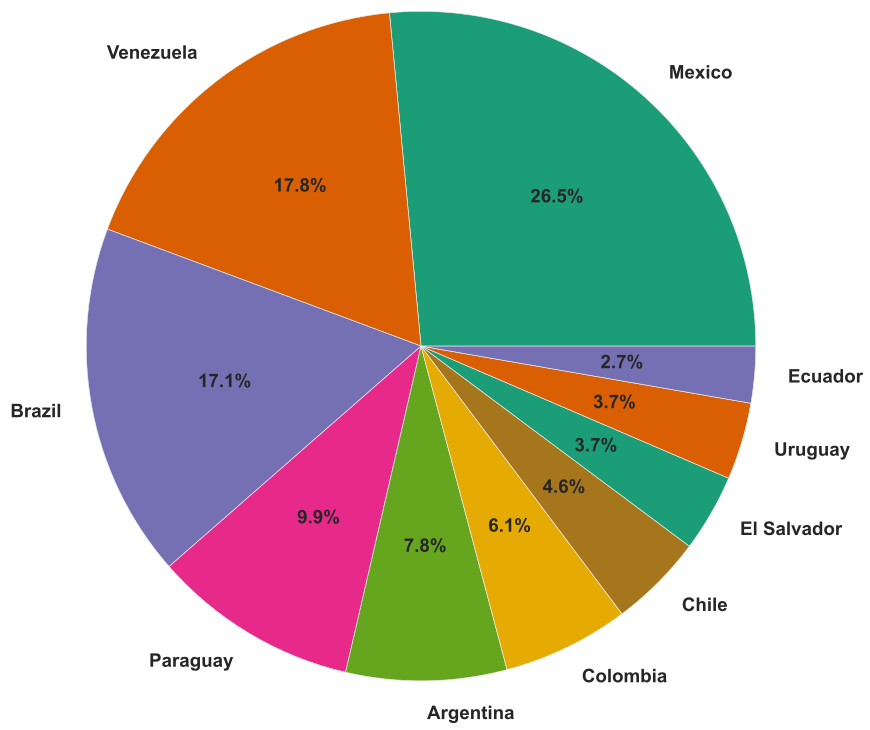
\includegraphics[width=\textwidth]{gsr_distribution}
%        \label{fig:gsrdistribution}
%        \caption{GSR Distribution From 2012-11 to 2014-03}
%    \end{subfigure}
%
%    \begin{subfigure}[b]{0.3\textwidth}
%        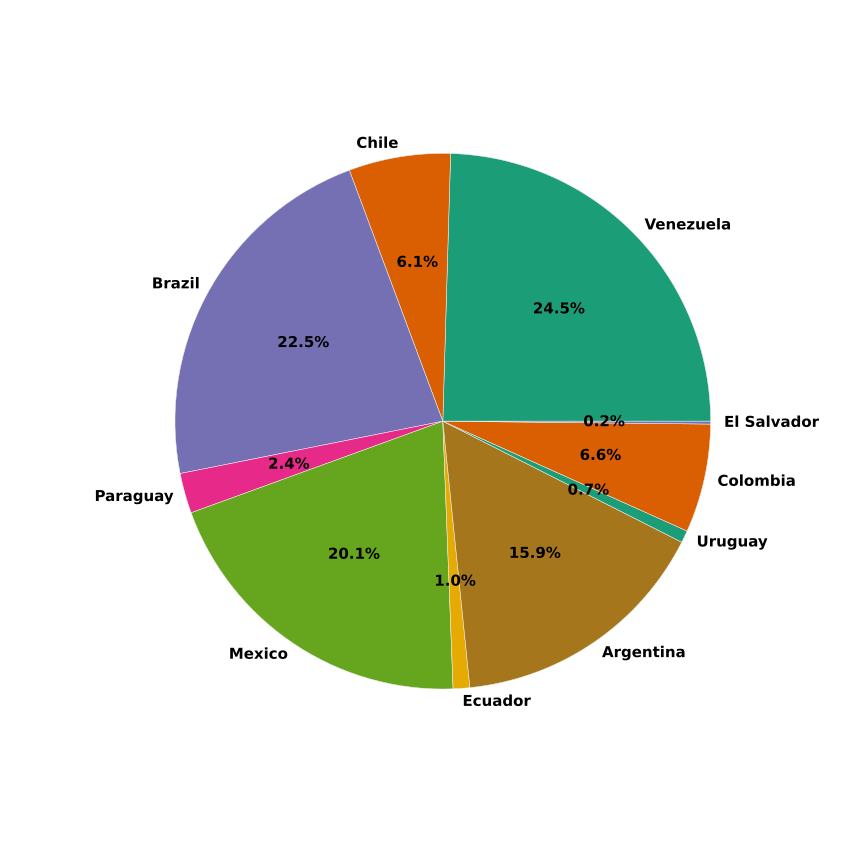
\includegraphics[width=\textwidth]{pp_dist}
%        \label{fig:ppdistribution}
%        \caption{Alerts Distribution From 2012-11 to 2014-03}
%    \end{subfigure}
%\end{figure*}


\begin{figure}
    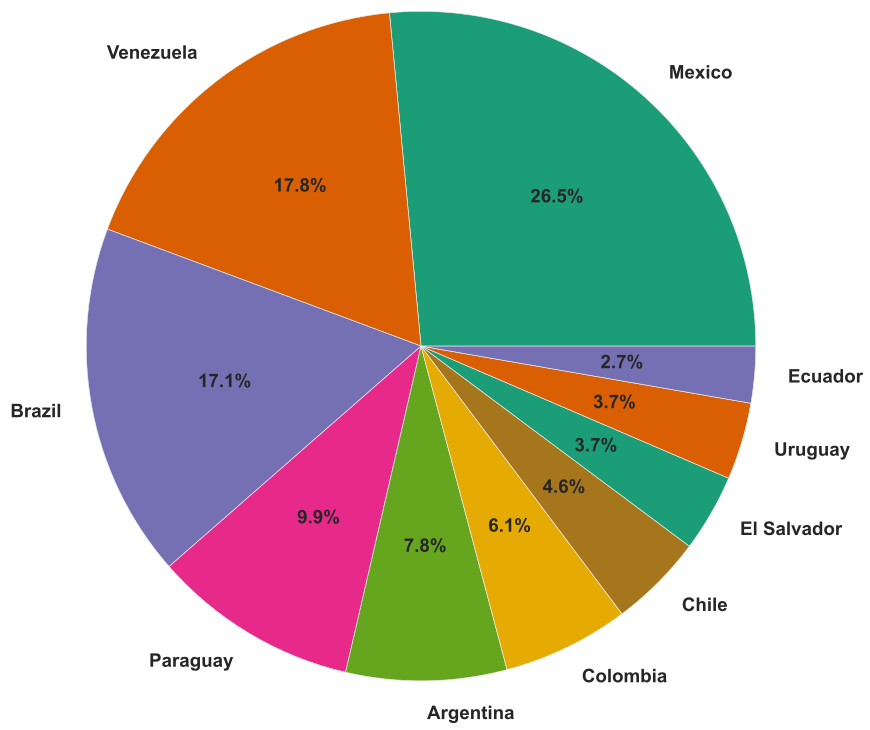
\includegraphics[width=.5\textwidth]{gsr_distribution}
    \label{fig:gsrdistribution}
    \caption{GSR Distribution From 2012-11 to 2014-03}
\end{figure}

\begin{figure}
    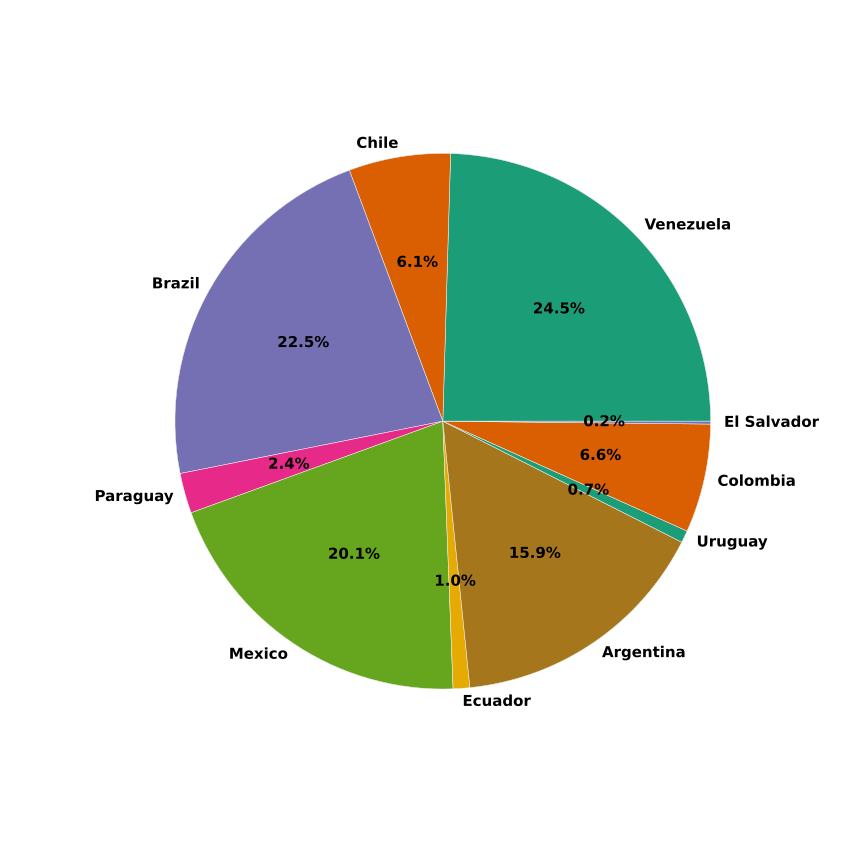
\includegraphics[width=.5\textwidth]{pp_dist}
    \label{fig:ppdistribution}
    \caption{Alerts Distribution From 2012-11 to 2014-03}
\end{figure}

\begin{figure}
    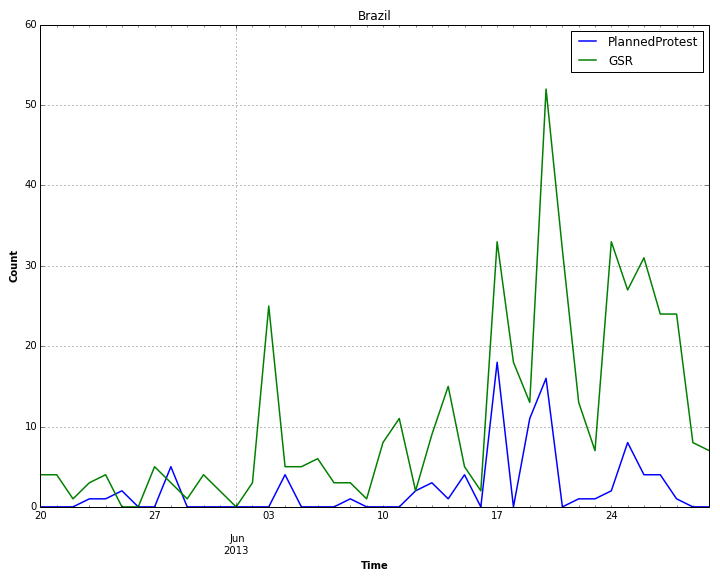
\includegraphics[width=0.5\textwidth]{brazil_june}
    \label{fig:brazil_june}
    \caption{Brazil June Protests}
\end{figure}

%\begin{figure*}
%    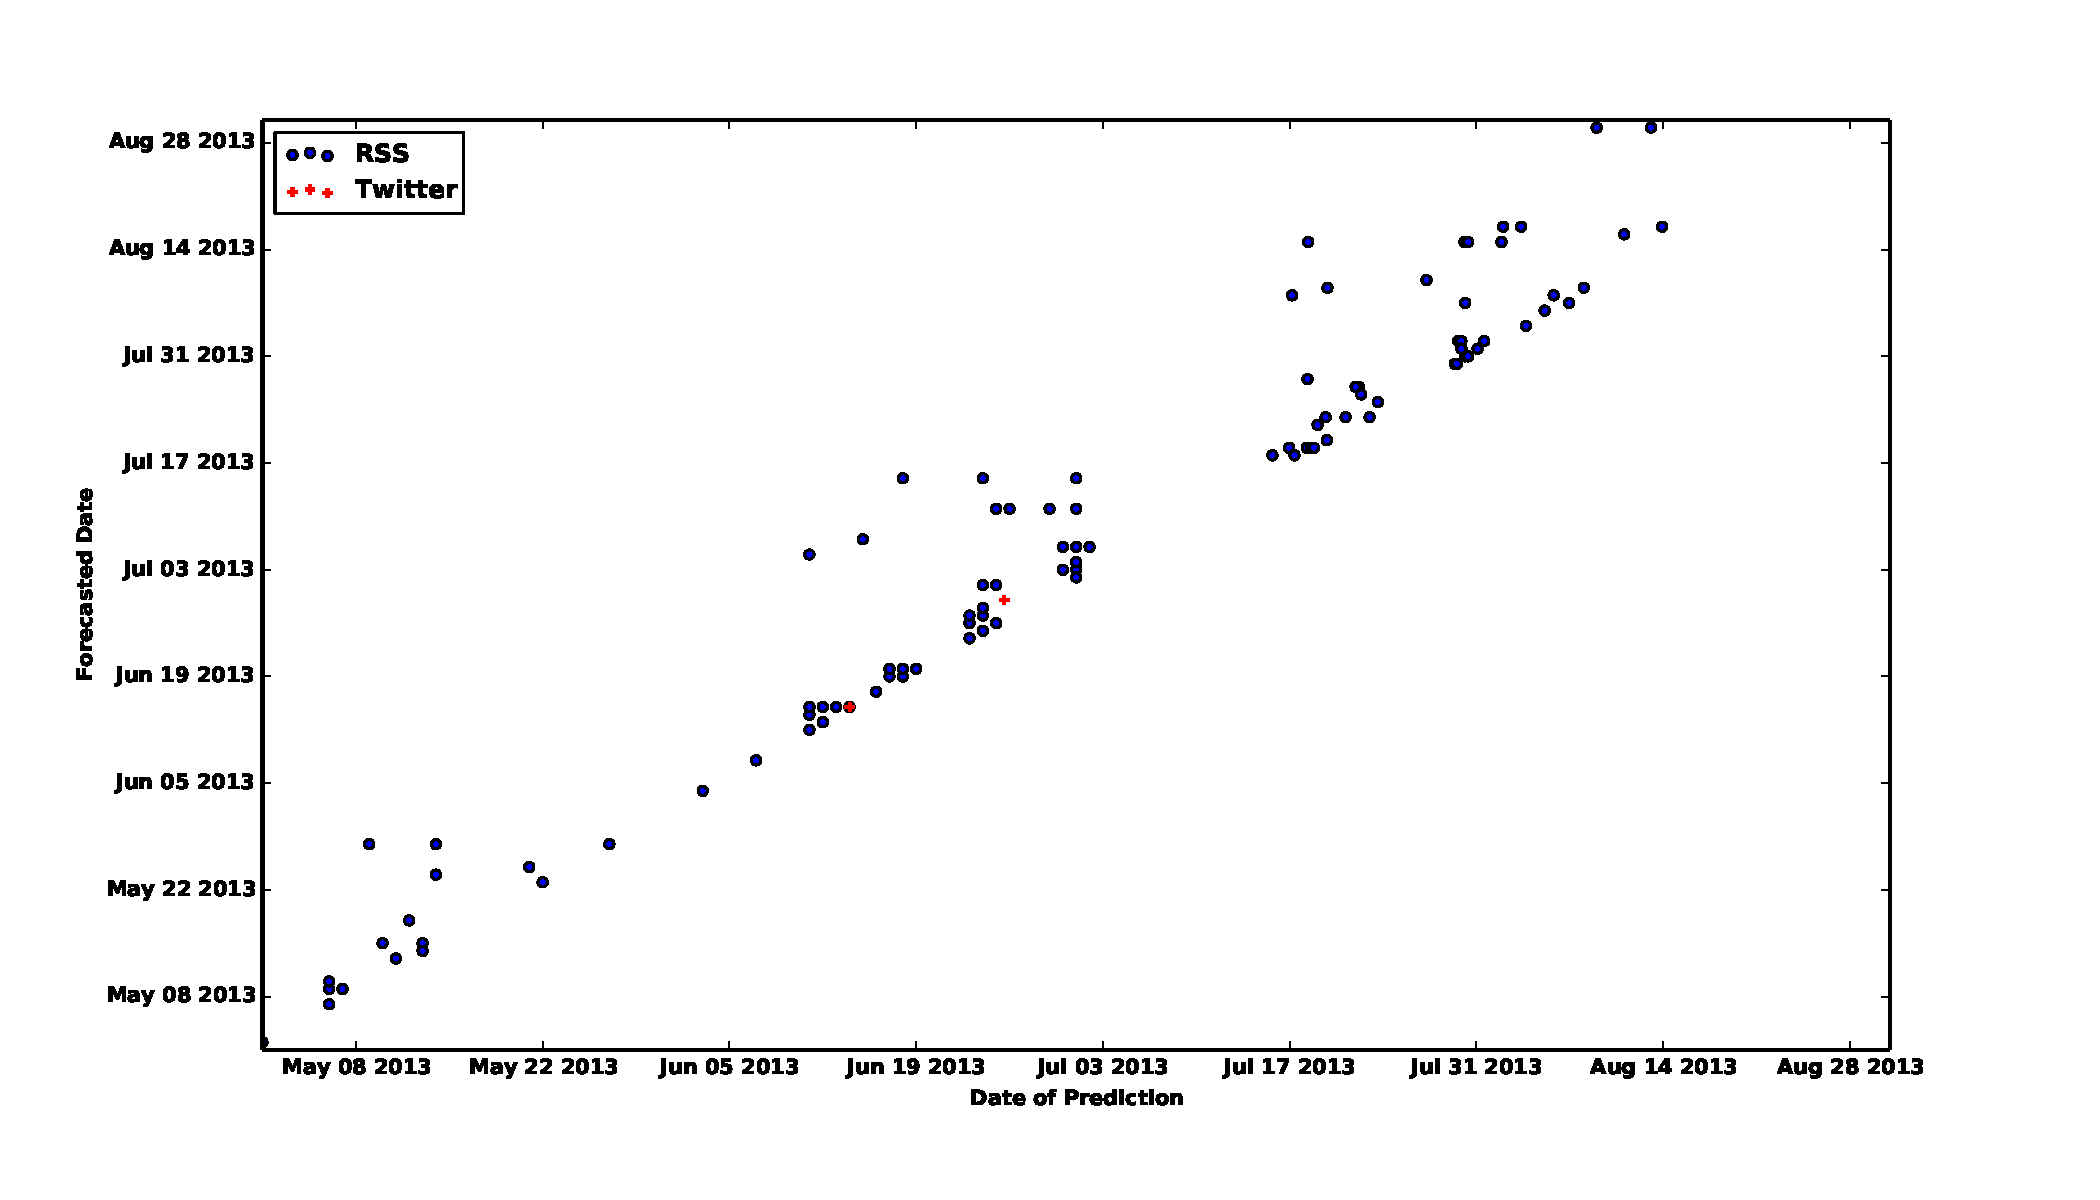
\includegraphics[width=\textwidth]{eventDateVsDate_brazil}
%    \caption{Date of Prediction vs Forecasted Date Brazil}
%    \label{fig:leadtime_brazil}
%\end{figure*}
%
%\begin{figure*}
%    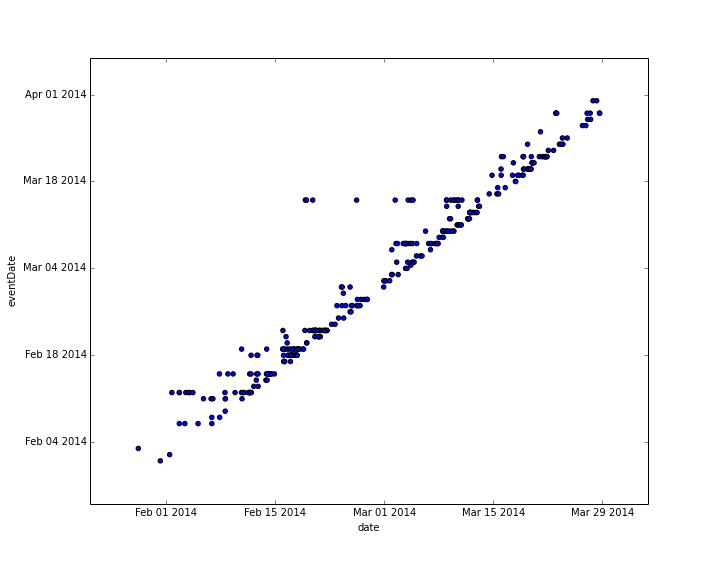
\includegraphics[width=\textwidth]{eventDateVsDate_venezuela}
%    \caption{Date of Prediction vs Forecasted Date Venezuela}
%    \label{fig:leadtime_venezuela}
%\end{figure*}

\begin{figure}
    
\includegraphics[width=0.5\textwidth]{monthlyqs}
    \caption{QS over the months}
    \label{fig:monthlyqs}
\end{figure}

\begin{figure}
    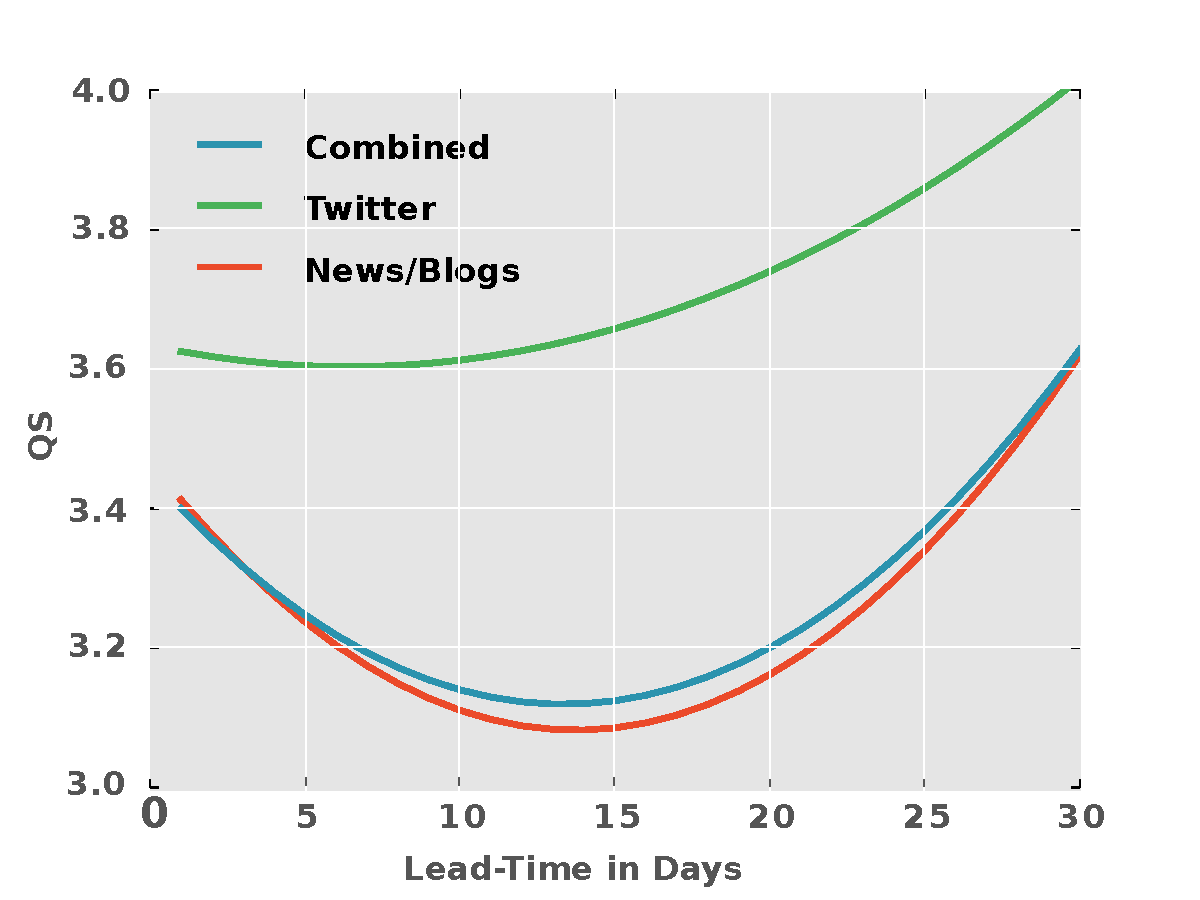
\includegraphics[width=0.5\textwidth]{leadTimeVsQS}
    \caption{Lead-Time vs Quality Score}
    \label{fig:leadTimeVsQS}
\end{figure}

\begin{figure}
    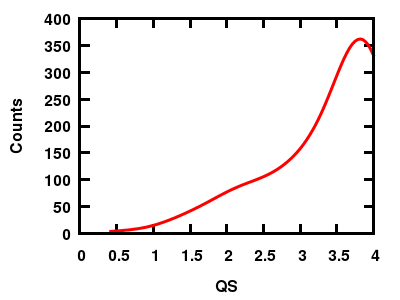
\includegraphics[width=0.5\textwidth]{doubleHump}
    \caption{QS Distribution}
    \label{fig:doubleHump}
\end{figure}

\begin{figure}
    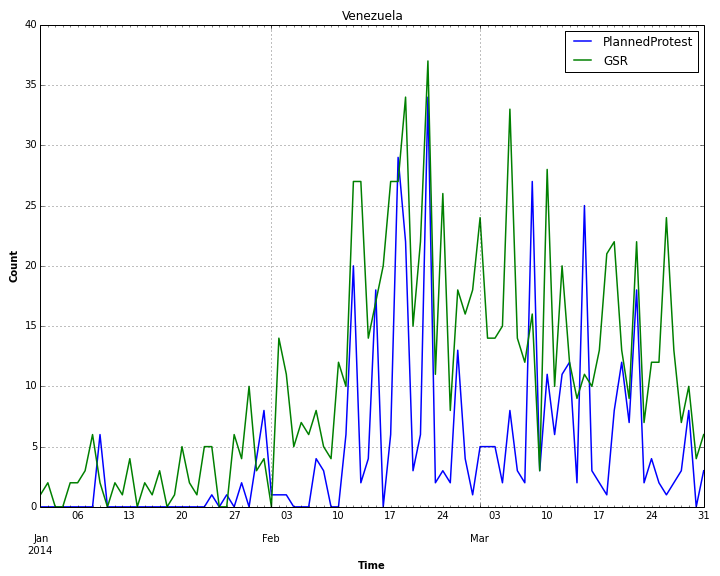
\includegraphics[width=0.5\textwidth]{venezuela}
    \label{fig:venezuela_feb}
    \caption{Venezuelan Protests}
\end{figure}

\begin{figure}
    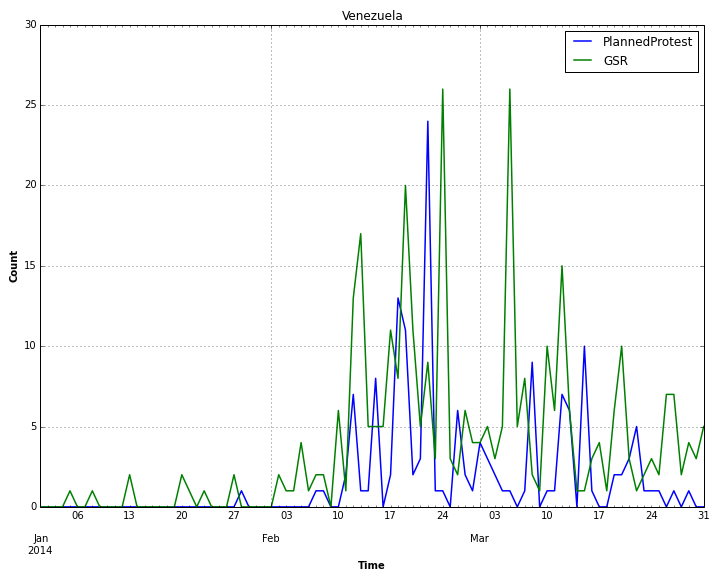
\includegraphics[width=0.5\textwidth]{venezuela_violent}
    \label{fig:venezuela_violent}
    \caption{Venezuelan Violent Protests}
\end{figure}

\begin{figure}
    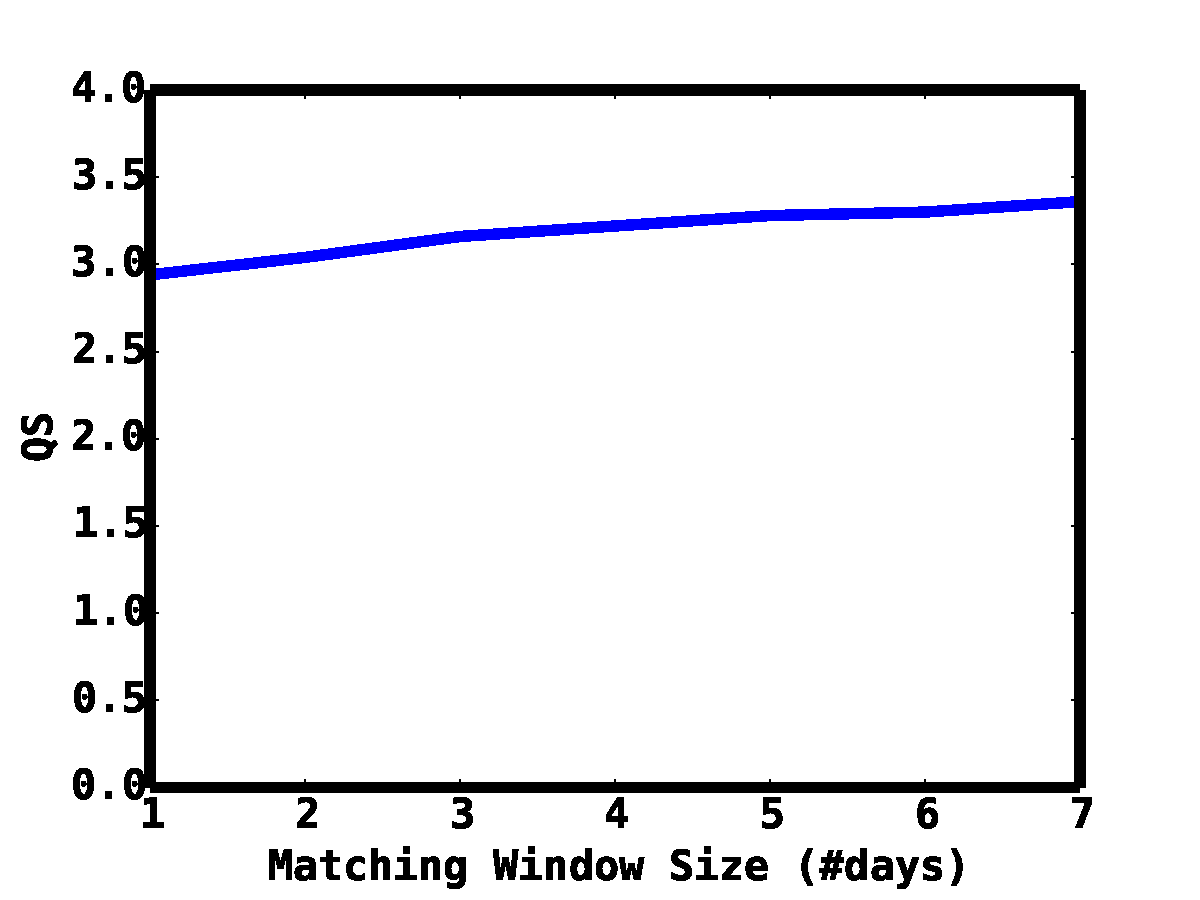
\includegraphics[width=0.5\textwidth]{matchingwindow}
    \label{fig:matchinginterval}
    \caption{QS vs Matching Interval Trade-Off}
\end{figure}










%\begin{figure}
%    \centering
%    \begin{subfigure}[b][0.3\textwidth]
%        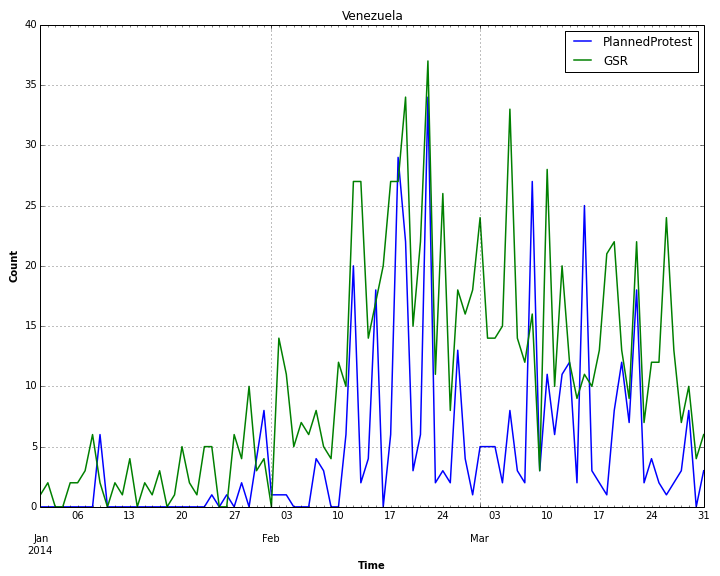
\includegraphics[width=\textwidth]{venezuela.png}
%        \caption{Venezuelan Protests}
%        \label{fig:Venezuela_feb}
%    \end{subfigure}
%    \begin{subfigure}[b][0.3\textwidth]
%        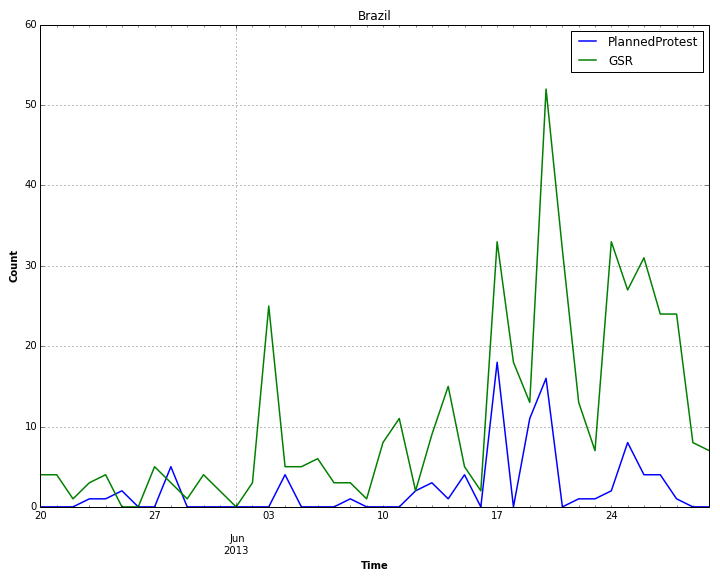
\includegraphics[width=\textwidth]{brazil_june.png}
%        \caption{Brazilian Riots in June}
%        \label{fig:Brazil_june}
%    \end{subfigure}
%\end{figure}
